% Capability Exposure Accounting, version 2.0.0. Compiler: pdfLaTeX; bibliography: BibTeX.
\documentclass[pdflatex,sn-mathphys-num]{sn-jnl}
\usepackage[T1]{fontenc}
\usepackage[utf8]{inputenc}
\usepackage{amsmath,amssymb,amsfonts}
\usepackage{graphicx,booktabs,tabularx,array,longtable}
\usepackage{fvextra,tikz,xurl,needspace}
\usetikzlibrary{arrows.meta,positioning}
\theoremstyle{plain}
\newtheorem{theorem}{Theorem}
\newtheorem{lemma}[theorem]{Lemma}
\newtheorem{proposition}[theorem]{Proposition}
\newtheorem{corollary}[theorem]{Corollary}
\theoremstyle{definition}
\newtheorem{definition}[theorem]{Definition}
\newcommand{\Cl}{\operatorname{Cl}}
\newcommand{\F}{\mathbb{F}}
\newcommand{\Adv}{\operatorname{Adv}}
\newcommand{\pk}{\mathsf{pk}}
\newcommand{\sk}{\mathsf{sk}}
\newcommand{\code}[1]{\texttt{#1}}
\newcolumntype{Y}{>{\raggedright\arraybackslash}X}
\emergencystretch=2em
\hypersetup{hidelinks,bookmarksdepth=2,pdftitle={Capability Exposure Accounting for Threshold-Based Encrypted Backup Recovery},pdfauthor={Samarjeet Malik and Shaurya Pratap Singh}}
\begin{document}
\raggedbottom
\title[Capability Exposure Accounting]{Capability Exposure Accounting for Threshold-Based Encrypted Backup Recovery}
\author[1]{\fnm{Samarjeet} \sur{Malik}}
\author[2]{\fnm{Shaurya Pratap} \sur{Singh}}
\affil[1]{\orgname{Ashoka University}}
\affil[2]{\orgname{Indian Institute of Science}}
\abstract{Deleting a custodian's local secret need not revoke an encrypted backup's recovery capability: copied credentials, recorded capsules, refreshed sharings and independent archive authorities can preserve access. We formalize this distinction using a typed capability closure coupled to finite-field observations. The model separates symbolic linear reconstruction from information leakage; a rank condition characterizes value-independent privacy for the declared linear view, including adaptive observation choices. Minimal erasure sets are characterized by hitting all surviving reconstruction or privacy witnesses, with immutable copies yielding explicit impossibility cases. A temporal specialization characterizes independently randomized sharing generations and explains why renewing shares and renewing their recipient credentials are different operations. The familiar deletion-receipt bound becomes a single-generation special case, and joint recovery, approval, deletion and log-quorum constraints expose the cost of additional outages. We validate the algebra against 7,407 finite matrices, retain the earlier baseline checks, explore eight temporal scenarios, and check four finite TLA+ lifecycle configurations. These cover 316,332 reachable states across separate runs; unsafe variants produce counterexamples for stale responses, premature receipts, rollback and request mismatch. An executable reference kernel adds scheduled concurrency and crash tests. The characterization is relative to declared symbolic operations and affine observations. It is neither a new cryptographic primitive nor a complete concrete-client confidentiality theorem or physical-erasure certification.}
\keywords{Capability exposure, encrypted backup, threshold recovery, cryptographic erasure, linear secret sharing, TLA+}
\maketitle


\section{Introduction}\label{sec:intro}

Encrypted recovery creates durable access to data whose live communication keys may already have evolved. Losing every message device is recoverable only if some external capability survives. Erasing access to an old record requires that the adversary's permitted later view contain no sufficient surviving path. These are different questions: legitimate recoverability is a property of available honest authorities, whereas confidentiality after compromise concerns the authority and material actually disclosed to the adversary.

Several distinctions determine the outcome. A record's birth epoch is unchanged when it is placed in a newer snapshot. Deleting a cached share does not remove a recorded share capsule's recipient key. Deleting an honest device's key does not remove a previously copied key. Refreshing sharing polynomials does not renew the credentials that decrypt their capsules. An independent archival service adds a recovery route rather than removing the ordinary route's limitations. Finally, an authentic approval can still authorize an attacker-controlled recipient through a genuine mistake.

The underlying mechanisms are established. Revocable backup and ephemerizer systems already exploit deliberate key destruction~\cite{boneh1996,perlman2007}; proactive sharing and CODEX address distributed custody under explicit compromise assumptions~\cite{herzberg1995,zhou2005,marsh2004}. CKS and GKP give cryptographic treatments of persistent key access~\cite{dodis2024,dodisstandard2024,backendal2026}. Our question is how to represent their surrounding lifecycle obligations without treating an individual guardian's status as the security state of the entire recovery system.

We organize the analysis around three research questions:
\begin{description}
\item[RQ1: Capability accounting.] Which surviving capabilities, including alternate and recorded paths, suffice for reconstruction or information leakage after a specified exposure?
\item[RQ2: Temporal exposure.] What changes when recipient credentials are copied across epochs, when sharing generations are independently refreshed, or when their delivery credentials are renewed?
\item[RQ3: Joint progress.] Which parameter and service conditions permit reconstruction, approval, deletion progress and ordered policy operation despite withholding and additional outages?
\end{description}

Our contribution is an explicit analysis interface and its checked lifecycle, rather than a new encryption construction. A monotone typed rule system represents conjunctive decryption and derivation dependencies. A linear module accounts for jointly exposed sharing observations, including correlations across generations. We prove closure and privacy characterizations relative to those declared operations; characterize deletion as hitting the appropriate minimal witnesses; and specialize the model to independently randomized threshold sharings. The specialization recovers the elementary single-generation deletion bound and also identifies cases for which per-generation holder counts are insufficient.

The distinction between reconstruction and privacy is central. Observing $S_0+S_1$ need not linearly reconstruct either seed, but it exposes a relation between them. A statement that the adversary cannot reconstruct a complete seed is therefore insufficient as a general confidentiality definition. We use separate predicates, and require the stronger privacy predicate whenever the claim concerns a value-independent sharing view.

We additionally specify a generation-aware release/expiry machine, give a manual inductive safety argument, and execute TLC on finite configurations and unsafe mutations. A reference implementation tests the critical queue, ownership-transfer and crash ordering. These forms of evidence remain separate from encryption security: we state a precise independent-slot component game, but make no completed end-to-end client-refinement claim. The formal results use familiar monotone-derivation, linear-sharing and witness-hitting ideas; no priority claim for those mathematical foundations is made~\cite{karchmer1993}.

\section{Position relative to prior work}\label{sec:related}

\paragraph{Deletion and custody.}
Boneh--Lipton's revocable backups and Perlman's temporal ephemerizers are direct predecessors to cryptographic forgetting and externally held temporary keys~\cite{boneh1996,perlman2007}. FadeVersion addresses assured deletion amid dependencies between retained versions and shared data, with a prototype evaluated on cloud storage~\cite{rahumed2011}. Our witness model represents dependencies and immutable copies explicitly; it does not establish the first backup-deletion architecture or reproduce FadeVersion's performance. The implementation here is a lifecycle reference, not a competing cloud-backup system.

Shamir/Pedersen sharing supplies the algebraic basis~\cite{shamir1979,pedersen1991}. Proactive sharing and APSS explicitly bound compromise over refresh windows and transitions~\cite{herzberg1995,zhou2005}. CODEX combines authorized secret distribution, Byzantine quorums and proactive techniques~\cite{marsh2004}. Our temporal theorem describes the complete historical linear view under stated independence conditions. It is not a replacement for an active distributed-refresh protocol: a clean reconstructor and independent coefficients alone do not implement APSS's transition guarantees.

\paragraph{Compact and evolving persistent keys.}
ROM-CKS has line and interval constructions, with preservation of compatible application security rather than an unrestricted key-indistinguishability promise~\cite{dodis2024}. Its adaptive simulation uses noncommitting techniques. The standard-model follow-up proves that the original general preservation objective cannot be instantiated as stated in that model, and instead recovers derived keys, restricts delegation and gives selective-security definitions~\cite{dodisstandard2024}. It is incorrect to treat this as only a change of hash assumption: the recovered functionality and admissible applications differ. Our independent-slot array is a less compact component with direct exposure accounting. It is not a standard-model substitute achieving CKS's full original functionality.

GKP/Grappa provides persistent interval access and post-compromise evolution under its specified group model~\cite{backendal2026}. The inspected full-version proof of Theorem 6.1 announces its oracle-query sequence in advance and uses honestly generated control messages. This differs from our arbitrary lifecycle scheduling with abstract verified certificates; it does not imply that our paper supplies a stronger cryptographic protocol theorem. Our results concern declared capability closure, affine views, and local release/expiry safety. They could serve as an audit layer around a persistent-key scheme, but no generic composition with CKS or GKP is proved.

\paragraph{Authentication, recovery and cloud-storage models.}
Kintsugi uses password-authenticated threshold recovery and an asynchronous model. Its inspected threat model assumes non-Byzantine nodes, permits honest-but-curious collusion and bounds share disclosure per refresh interval~\cite{ma2025}. Translating notation, its reconstruction threshold is one greater than its collusion parameter. Its password-authentication question differs from whether old recipient credentials or archive paths survive a later erasure barrier. Our human-approval profile does not inherit its password-guessing guarantees.

Janneck--Riepel refines encrypted cloud-storage security with adaptive corruption, authentication modularity, and a network-adversary model whose registration exception matters~\cite{janneck2026}. The authors' primary record supports those model-level comparisons; we do not claim an independent audit of their full reduction. Our trusted bootstrap and verified log are assumed services, not substitutes for their network-authentication proof. Lifecycle counterexamples here do not demonstrate a break of their scheme or a cryptographic separation from it. SafetyPin and SVR3 provide implemented recovery with hardware-based trust splitting and deployment-specific protection~\cite{dauterman2020,connell2024}; our software reference has no corresponding deployment or hardware-erasure evidence.

\begin{table}[htbp]
\caption{Required persistent-key comparison dimensions. Properties refer to the cited interfaces; ``relative'' denotes the declared ideal operations, not an end-to-end cryptographic guarantee.}\label{tab:comparison}
\centering\footnotesize
\begin{tabularx}{\linewidth}{@{}p{.20\linewidth}YYY@{}}\toprule
Dimension & ROM-CKS / standard-model CKS & GKP / Grappa & This analysis / slot baseline\\\midrule
Storage & Compact; original line constant state, interval logarithmic state; follow-up graph-dependent constructions & Compact interval and group state & $O(T)$ slots per guardian; analysis graph need not be compact\\
Erasure scope & Permitted forgetting families; follow-up derives keys rather than original seeds & Interval progression and rotation under specified cleanness & Explicit birth-epoch/generation paths and allowed exposure map\\
Recovery & Original seeds versus derived keys, depending on definition & Persistent group access within intervals & External threshold restoration with stated surviving factors\\
Security model & Preservation in ROM versus modified standard-model selective key security & Inspected nonadaptive, passive control-message theorem & Exact symbolic/linear results; component cryptography and abstract services\\
Forward security & Application/interface-specific forgetting & Instantiation and interval-policy dependent & Independent erased-slot lemma; actual path cleanup required\\
Future state exposure & Compatibility and fresh application input determine recovery & Group/interval healing conditions & Exposed bank includes future slots until recipient paths are renewed\\
Adaptive corruption & ROM adaptive simulation; follow-up explicitly selective & Preannounced sequence in inspected proof & Adaptive linear observations; no full adaptive ciphertext-composition theorem\\\bottomrule
\end{tabularx}
\end{table}

The gap addressed is thus a specification and analysis obligation: the surrounding system must account for every declared source of a usable observation and enforce the lifecycle order on which that accounting relies. The results here do not assert that the cited constructions cannot be extended to satisfy that obligation. The novelty of a general-purpose audit method would require broader external validation; the present contribution is bounded by the explicit model and evidence below.


\section{Capability and observation semantics}\label{sec:model}

\subsection{State, locations and compromise}
A record has immutable birth epoch $e$. Its sharing generations $g$ may change without changing $e$. Snapshot version $v$ is a container identifier, not a birth epoch. Let $j$ be the committed recovery frontier, $W$ an ordinary retention window, and $L$ the effective deletion floor. Ordinary recovery covers promised records with $j-W+1\le e\le j$; advancing $j$ requires completed barriers for older protected records. These are epoch-count guarantees unless a separate timing contract supplies deadlines.

At time $t$, write the system state as $(H_t,A_t,P_t,\Pi_t,J_t)$: honest located capabilities, adversary-owned knowledge, public recorded material, lifecycle/policy state, and pending work. The atom universe $V$ uses tags for role, location, epoch, generation, holder and bank version. Honest locations and adversary copies are distinct origins that may derive the same usable key value. Deletion removes an honest origin; it never removes a copied value from $A_t$. Once a capsule or response is recorded, deleting an honest replica does not remove the adversary's record.

The exposure map specifies which honest locations a corruption or later snapshot discloses. It is not assumed that every surviving legitimate recovery authority is simultaneously available to the adversary. An ordinary-compromise claim may exclude an independent archive authority, whereas a claim about erasure across all recovery routes must include it. This choice is part of the experiment, not an implicit exception after an attack.

We distinguish four compromise interfaces. \emph{Identity compromise} supplies signing authority and malicious voting behavior, without automatically supplying a data slot. \emph{Device compromise} supplies the enumerated local slots, caches, buffers and retained wrappers. \emph{Capability disclosure} supplies a particular copied pair, slot, response or derivation ancestor without necessarily controlling an identity. \emph{Recovery-authority compromise} supplies an alternate route such as an archive key or reconstructed client seed. The adversary's copies are monotone under all later honest operations.

The lifetime identity budget $f$ is scoped to one configuration for approval/log claims. The historical bound $c_{e,g}$ counts distinct otherwise-erased honest indices with useful copied paths at the selected barrier/observation for that epoch and generation. It does not reset an attacker's memory at refresh. A copied credential may contribute to several $c_{e,g}$ values. Our retained baseline BFS uses the stricter budget on every copied honest slot in a trace prefix; that exploration is not claimed equivalent to every exposure schedule permitted by the theorem.

\subsection{Declared symbolic operations}
Let $\mathcal R$ contain typed rules $Q\Rightarrow v$, where the premise set $Q\subseteq V$ is conjunctive. A recorded capsule \emph{and} its matching private slot derive a share observation. A wrapped slot \emph{and} its wrapping root derive that slot. A cached pair, exposed sender buffer, or delivered response can independently supply an observation. An archive capsule and its archive key derive the seed. A seed and an encrypted record derive a record-decryption capability. A signing identity alone is not a decryption rule.

Accessible observation atoms index rows of a matrix over a prime field. The closure adds all conclusions of enabled rules and any registered seed atom obtainable by a linear combination of accessible rows. It repeats until a least fixed point $\Cl_{\mathcal R}(K)$ is reached. A linear decoder is part of the declared operation language, not an assertion that all possible nonlinear algorithms have been enumerated.

\begin{theorem}[Relative closure characterization]\label{thm:closure}
For a finite atom universe and fixed typed rules/linear decoders, $v\in\Cl_{\mathcal R}(K)$ if and only if $v$ has a finite derivation from $K$ using those operations. The naive fixed-point procedure terminates after at most $|V|$ productive rounds.
\end{theorem}
\begin{proof}
Every added Horn conclusion has a proof from already derived premises. Every linear-decoder step has a row-combination certificate, so induction over productive rounds gives soundness. Conversely, induction over a finite derivation tree places its root in the fixed point: every premise is eventually present and its operation is enabled. Each productive round adds at least one atom, proving termination.
\end{proof}

Completeness is relative to the inventory. Applying the result to a concrete backup requires that every relevant exposure and derivation be represented. Neither an unlisted disk root nor an unmodeled client side effect is excluded by calling the model complete. Authorization transitions supply response facts only when the separately specified state machine emits them.

\begin{figure}[htbp]
\centering
\resizebox{\linewidth}{!}{%
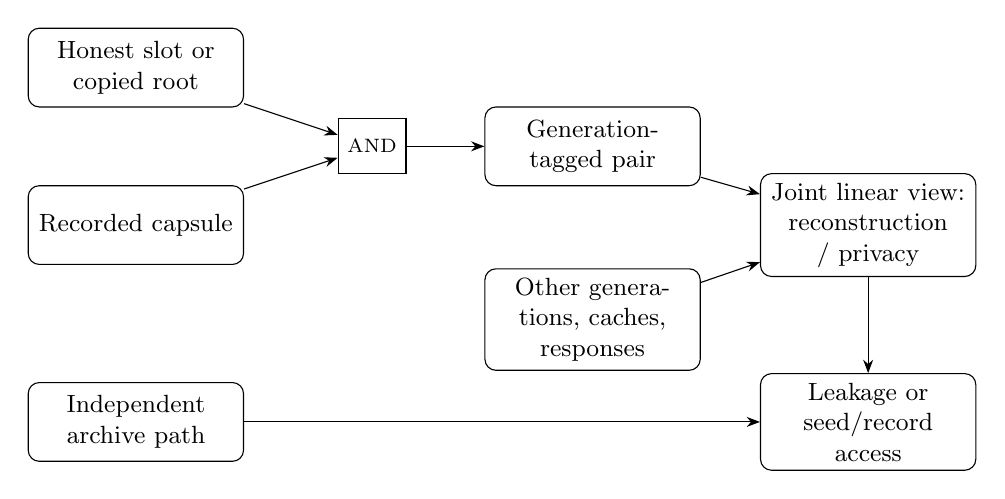
\begin{tikzpicture}[>=Stealth,box/.style={draw,rounded corners,align=center,font=\small,text width=25mm,minimum height=10mm},gate/.style={draw,rectangle,align=center,font=\scriptsize,minimum size=7mm}]
\node[box] (root) at (0,4.5) {Honest slot or copied root};
\node[box] (cap) at (0,2.5) {Recorded capsule};
\node[gate] (and) at (3,3.5) {AND};
\node[box] (pair) at (5.8,3.5) {Generation-tagged pair};
\node[box] (obs) at (5.8,1.3) {Other generations, caches, responses};
\node[box] (linear) at (9.3,2.5) {Joint linear view: reconstruction / privacy};
\node[box] (archive) at (0,0) {Independent archive path};
\node[box] (seed) at (9.3,0) {Leakage or seed/record access};
\draw[->] (root)--(and);\draw[->] (cap)--(and);\draw[->] (and)--(pair);
\draw[->] (pair)--(linear);\draw[->] (obs)--(linear);\draw[->] (linear)--(seed);
\draw[->] (archive)--(seed);
\end{tikzpicture}}
\caption{A capability hypergraph, not ordinary edge reachability. Conjunctive openings feed a joint observation module. An immutable copied root preserves its derivation despite honest deletion. Archive paths may bypass the ordinary sharing module. The module's reconstruction and privacy predicates are distinct.}\label{fig:capabilities}
\end{figure}

\subsection{Reconstruction and privacy are different predicates}
Let $S\in\mathcal D_1\times\cdots\times\mathcal D_k$ contain protected seed parameters, with each domain containing at least two field elements. Repeated generations of the same seed use the same coordinate. Let $R$ be an independent uniform vector of sharing/blinding coefficients over $\F_p$. For a fixed public operation choice, the accessible linear view is
\begin{equation}\label{eq:view}
 Y=A S+B R.
\end{equation}
All observation sources and public affine observations must be included. For privacy of a target subset conditioned on other seeds, their values are supplied to closure and their known contribution is subtracted; unknown nonuniform seeds are not silently treated as uniform masks.

\Needspace{12\baselineskip}
\begin{theorem}[Linear reconstruction and value-independent privacy]\label{thm:rank}
For the declared linear layer: (i) a seed coordinate is linearly reconstructible exactly when its unit row is in the row span of $[A\ B]$; (ii) the distribution of $Y$ is independent of all protected seed values exactly when
\begin{equation}\label{eq:privacy}
 \operatorname{rank}[B\ A]=\operatorname{rank}B.
\end{equation}
The privacy claim applies to arbitrary embedded seed domains as above. The reconstruction claim concerns linear decoders; with arbitrary bounded seed encodings, absence of its row-span witness does not rule out every nonlinear decoder.
\end{theorem}
\begin{proof}
A row-span representation gives a linear combination returning the selected coordinate; a linear decoder valid on all field inputs must have that coefficient row. For privacy, uniform $R$ makes $Y$ uniform on the coset $A s+\operatorname{im}B$. All these distributions agree if every column of $A$ lies in $\operatorname{im}B$. Conversely, changing only one seed between two distinct allowed values gives a nonzero scalar multiple of that column. Equality of cosets forces the column into $\operatorname{im}B$. Column containment is equivalent to~\eqref{eq:privacy}.
\end{proof}

For example, $Y=S_0+S_1$ with no masks linearly reconstructs neither coordinate but leaks their relation, violating joint privacy. Embedded domains can make such leakage even stronger. A deletion analysis must therefore name its predicate: preventing full linear reconstruction is weaker than preserving a value-independent view.

\begin{corollary}[Adaptive observations]\label{cor:adaptive}
Suppose observation choices depend only on the visible prefix, public seed-independent data, and fixed adversary coins. For each terminal transcript passing~\eqref{eq:privacy}, its probability mass is identical for every allowed seed vector. This is a statement about the accepted subdistribution, not conditioning on a potentially challenge-dependent freshness event.
\end{corollary}
\begin{proof}
Fix a terminal transcript and seed difference $\Delta$. The rank condition provides $d$ with $Bd=-A\Delta$. Translating the original uniform mask tape by $d$ while changing $S$ by $\Delta$ preserves every recorded answer. It therefore preserves every adaptive row choice and the entire transcript. Translation bijects the transcript fibers and preserves their probability mass. Public metadata or nonlinear observations omitted from~\eqref{eq:view} are outside the premise.
\end{proof}

\subsection{Erasure as witness elimination}
Fix public recorded facts $P$, immutable adversary copies $A_0$, and honest-origin facts $H$ eligible for the stated future snapshot. A permitted deletion $D\subseteq H$ leaves view roots $P\cup A_0\cup(H\setminus D)$. For either selected bad predicate $F$---declared reconstruction or failure of~\eqref{eq:privacy} after closure---let $\mathcal W_F$ be the inclusion-minimal supports $W\subseteq A_0\cup H$ for which $F(P\cup W)=1$.

\begin{theorem}[Witness-hitting characterization]\label{thm:cuts}
A permitted deletion prevents the selected bad predicate if and only if it intersects every support in $\mathcal W_F$. If a witness has no permitted honest-origin element, no allowed deletion can establish the selected property.
\end{theorem}
\begin{proof}
Both predicates are monotone under additional knowledge. A surviving unhit witness certifies failure. Conversely, if failure survives deletion, finiteness permits removal of redundant roots until a minimal surviving witness remains; it was not hit. An immutable witness cannot be hit by any permitted deletion.
\end{proof}

Thus a minimum-weight deletion can be formulated as a hitting-set optimization over witness supports. This is a standard monotone-access-structure formulation, not a new ordinary graph min-cut theorem. Threshold reconstruction and conjunctive decryption prevent replacement by simple edge reachability. Our exact implementation enumerates supports and deletions; no polynomial optimization guarantee is claimed. Privacy witnesses, rather than reconstruction witnesses, are required for a privacy promise: in the sum example, removing no facts already prevents linear recovery of $S_0$, but removing the sum observation is necessary for joint privacy.

\subsection{Independent generations and copied delivery credentials}
For epoch $e$, generation $g$ uses threshold $t_g$, distinct nonzero indices, and independently sampled polynomials
\begin{equation}\label{eq:sharing}
 A_g(X)=S_e+\sum_{i=1}^{t_g-1}a_{g,i}X^i,
 \qquad B_g(X)=\sum_{i=0}^{t_g-1}b_{g,i}X^i.
\end{equation}
Pedersen coefficient commitments are $g_0^{a_{g,i}}h_0^{b_{g,i}}$, with $a_{g,0}=S_e$. Their exponent representation, using $h_0=g_0^\beta$, is a stronger affine view; hiding that view suffices to hide the actual commitments. Let $I_g$ include every genuine share/opening pair obtainable across the full recorded history by that generation's capabilities, not only currently held shares.

\begin{theorem}[Joint independent-generation characterization]\label{thm:temporal}
Assume honest generation, mutually independent polynomial randomness, no extra coefficient/seed observations, and the declared capsule-opening interfaces. The joint commitment/opening view of any finite collection of generations of $S_e$ is independent of $S_e$ if and only if $|I_g|<t_g$ for every generation. This also holds on adaptive terminal transcripts satisfying those conditions.
\end{theorem}
\begin{proof}
For each subthreshold terminal set, the polynomial translation in Appendix~\ref{app:proofs} changes the common constant by the same $\Delta$ while preserving all that generation's commitments/openings. Independent random-coefficient blocks permit simultaneous bijective translations, preserving the joint adaptive transcript. If one generation exposes at least $t_g$ distinct pairs, interpolation returns $S_e$, so privacy fails.
\end{proof}

The rule layer determines $I_g$. Reused recipient keys may open old and future capsules; a captured bank can include future period slots even when the periods' keys were originally independent. Renewing recipient banks removes old-key rules to \emph{new} capsules but cannot remove prior observations. Refreshing an already known $S_e$ cannot restore its secrecy. Conversely, a fresh independent epoch seed can pass the target privacy test even conditioned on all old seeds when its renewed delivery paths and auxiliary disclosures leave the new view subthreshold.

Independence is essential. Reusing polynomial randomness across generations can produce a joint rank failure while every individual generation has fewer than $t_g$ disclosed points. Auxiliary coefficient leaks, correlated sharings, alternate authorities and changed thresholds must be analyzed with the general closure/rank condition, not the per-generation counting shortcut. These statements are not an active distributed proactive-sharing protocol.

\subsection{The single-generation deletion bound as a specialization}
With one generation and one useful point per index, suppose $q_d$ matching receipts include at most $f$ dishonest issuers, honest signers remove every local path, and $c$ otherwise-erased honest indices have useful prior copies. At least $\max(0,q_d-f)$ indices lose their honest paths; remaining indices plus prior copies give the tight worst-case bound
\begin{equation}\label{eq:deletion}
 m_{\max}=\min(n,n-q_d+f+c),\qquad
 q_d\ge n-t+f+c+1\ \Longleftrightarrow\ m_{\max}<t.
\end{equation}
Tightness places as many liars as possible among signers and copies at distinct honest erasers. The temporal theorem then supplies sharing-view privacy. This recovers the existing elementary result, but only for the stated single-generation/path assumptions. A signed receipt does not prove their physical truth.


\section{Reference protocol, assumptions and component security}\label{sec:protocol}

\subsection{Explicit exposure interfaces}
Table~\ref{tab:oracles} specifies the trace-level observations used by the analysis. An honest party's state and the challenger's private bookkeeping are distinct. The exposure inventory must enumerate storage wrappers, snapshots and volatile work; deletion of one named field is not proof that this inventory is exhaustive.

\begin{table}[htbp]
\caption{Trace interfaces and returned material. A real device disclosure may cross several compromise categories when keys are co-resident.}\label{tab:oracles}
\centering\footnotesize
\begin{tabularx}{\linewidth}{@{}p{.26\linewidth}Y@{}}\toprule
Interface & State or observation supplied\\\midrule
Setup / Publish & Honest bank directories, epoch/generation parameters, public manifests, commitments and recorded capsules\\
CopySlot$(h,b,e)$ & The present matching private slot, or failure if absent; an earlier copy remains in adversary state\\
CopyBankCapability & Every retained slot in that bank snapshot, including future periods; no signing authority is implied by this narrower interface\\
CorruptDevice & Enumerated stored slots, cached shares, wrapper roots and volatile responses; stored signing keys, if present, also count as identity compromise\\
CorruptIdentity & Specified signing/policy keys and malicious voting control, without inventing possession of a data slot\\
CopyPair / CopyResponse & The declared pair or recorded response-opening material; irreversible deliveries are never retracted\\
CorruptRecoverer & Its reconstructed seeds, available pairs, plaintext outputs, ephemeral session state and buffers\\
CorruptArchive & The specified independent archival root/slots and their recorded envelopes\\
Expire / Crash / Restart & Lifecycle transitions; receipts and public log metadata only. Old snapshots must pass the nonrollback anchor\\
FinalSnapshot & Exactly the honest-origin fields allowed by the experiment's exposure map, followed by declared closure\\\bottomrule
\end{tabularx}
\end{table}

The ideal seed-view game lets an adversary nominate two allowed seed vectors with identical public metadata, samples a hidden bit and uniform sharing masks, and answers adaptive declared observations. Recorded encryption envelopes are opaque symbols in this game. At the final observation it applies the rank-privacy freshness test; on accepted runs it outputs whether the guess equals the bit, and otherwise an independent fair bit. The advantage is always
\begin{equation}\label{eq:advantage}
 \Adv_{\mathrm{view}}(\mathcal A)=\left|\Pr[\mathsf{out}=1]-\tfrac12\right|.
\end{equation}
Corollary~\ref{cor:adaptive} gives zero advantage for the accepted linear-view subdistribution. This is a complete statement about that ideal experiment. It does not include concrete ciphertext leakage or arbitrary computations on restored challenge plaintext. A concrete historical-data game would require a separate refinement/composition theorem; this paper does not claim one. The earlier schematic protocol-level bound is therefore not retained as a theorem.

\subsection{A concrete classical profile}\label{sec:profile}
The selected profile uses independent 32-byte epoch seeds embedded in the scalar field of NIST P-384. The sharing prime is the group order, not the curve-coordinate prime (hexadecimal; concatenate the three lines):
\begin{Verbatim}[fontsize=\small]
FFFFFFFFFFFFFFFFFFFFFFFFFFFFFFFF
FFFFFFFFFFFFFFFFC7634D81F4372DDF
581A0DB248B0A77AECEC196ACCC52973
\end{Verbatim}
Scalars use 48-byte unsigned big-endian encodings strictly below that prime. Coefficients and blinders are uniform including zero. Holder indices are distinct nonzero elements, with profile limit $n\le255$. P-384 commitments use the standard generator and a second generator obtained with RFC~9380 suite \code{P384\_XMD:SHA-384\_SSWU\_RO\_}, message \code{h}, and domain tag \code{CEAB-v2-Pedersen-H}, retrying with an encoded counter for identity or $\pm g_0$~\cite{rfc9380,sec2}. The unknown generator relation is an assumption of this instantiation; it is not established by the toy algebra checker. Compressed commitment points occupy 49 bytes.

\begin{table}[htbp]
\caption{Concrete algorithm choices. Specifying the profile is separate from implementing or proving its complete composition.}\label{tab:profile}
\centering\footnotesize
\begin{tabularx}{\linewidth}{@{}p{.24\linewidth}Y@{}}\toprule
Component & Profile and binding requirements\\\midrule
Capsule PKE & RFC~9180 HPKE Base; DHKEM(X25519, HKDF-SHA256), KEM 0x0020; KDF 0x0001; ChaCha20Poly1305 AEAD 0x0003. Independent finite-bank slots; signed manifest supplies sender/context authentication~\cite{rfc9180}\\
Object PRF & HMAC-SHA256 under the uniform 32-byte epoch seed, over typed deterministic CBOR containing domain, account, creation configuration, birth epoch, object ID and immutable header\\
Data AEAD & ChaCha20-Poly1305; nonce is four zero bytes followed by the uint64 big-endian chunk index, never repeated under an object key. Profile limit $2^{32}-1$ chunks, at most 1 MiB each~\cite{rfc8439}\\
Signatures & Pure Ed25519 on SHA256 of a typed, domain-separated complete-message encoding; canonical validating verification. This is not Ed25519ph~\cite{rfc8032}\\
Hash and encoding & SHA-256; RFC~8949 core deterministic CBOR, definite lengths and bytewise encoded-key ordering. Reject duplicates, unsupported required fields, invalid scalars/points and oversized requests~\cite{rfc8949}\\
Private release & Short-lived authenticated TLS~1.3 with forward-secret ephemeral exchange, exporter binding to the approved recipient/request, no release in early data, and explicit session/buffer cleanup~\cite{rfc8446}\\\bottomrule
\end{tabularx}
\end{table}

Capsules contain exactly a share and blinder, 96 raw bytes. HPKE info binds account, configuration, bank, epoch, generation and holder; associated data additionally binds commitments, package identity and algorithms. The data header is immutable and authenticated. Random 32-byte object identifiers give collision probability at most $q(q-1)/2^{257}$ for $q$ independently sampled IDs. An uncertain interrupted creation is abandoned under a fresh identifier rather than reusing a key/nonce for changed plaintext. The overall profile targets approximately 128-bit classical strength, bounded by its weakest components; a 256-bit seed is not a blanket 256-bit security claim.

\subsection{Exact slot-component game and guessing losses}\label{sec:slots}
The slot game creates $nT$ independent labeled PKE pairs. It exposes every public key and permits recording all capsules before or after deletion. One challenge encrypts the adversary's equal-length pair under a selected guardian/period key. Other slots can be exposed completely. Labeled decryption queries are permitted except for the exact protected challenge. Freshness excludes every earlier target-slot disclosure, including a regenerating wrapper, secondary store or rollback image. A later snapshot contains only genuinely retained slots. Nonfresh outcomes use the fair-bit convention in~\eqref{eq:advantage}.

\begin{lemma}[Independent-slot component]\label{lem:slot}
Under the specified labeled IND-CCA PKE interface and actual target-slot erasure, a selective guardian/period challenge reduces to one PKE challenge without a slot-guessing factor. Selecting only the period adaptively among $T$ incurs at most $T$; selecting only the guardian among $n$ incurs at most $n$; selecting both among $nT$ incurs at most $nT$, with polynomial setup/query work.
\end{lemma}
\begin{proof}
Embed the PKE challenge public key at the selected or guessed pair and generate all other keys. The public directory has the honest independent distribution. Other-slot disclosures are answerable; target decryption queries go to the CCA oracle except the prohibited challenge. A fresh post-deletion snapshot never needs the unknown target secret. Premature target exposure or a wrong target guess yields an independent fair outcome. Uniformly guessing the unfixed coordinates supplies the stated factors.
\end{proof}

For a fixed target epoch, masking at most $n$ recipient capsules is a separate $n$-hop argument using selective-pair component challenges. If an outer experiment guesses one of $N$ epochs, its corresponding accounting is $Nn$, not $NnT$ when $N$ already enumerates the challenged periods. A guessed final useful-index set would introduce a separate partition loss; no such completed concrete-data reduction is asserted here. Independent data entropy alone cannot heal a stolen bank containing enough future slots.

\subsection{Operational assumptions and failure terms}
\begin{table}[htbp]
\caption{Assumptions, dependent statements and failure consequences.}\label{tab:assumptions}
\centering\footnotesize
\begin{tabularx}{\linewidth}{@{}p{.26\linewidth}YY@{}}\toprule
Assumption & Dependent result & If absent\\\midrule
Complete declared inventory and affine-view coverage & Closure/privacy application & An omitted wrapper or nonlinear client observation invalidates the application\\
Honest independently randomized sharing & Temporal specialization & Malicious/correlated generation requires another analysis\\
Actual honest cleanup, including wrappers and buffers & Post-barrier bound & A retained or resurrected path remains useful\\
Independent recipient slots & Slot component & Other-key exposure can recreate a target key\\
Authentic ordered log/checkpoints & Release ordering and policy & Replay, rollback or conflicting accepted states\\
External authentic bootstrap & Identity recovery & Cloned/replaced authority can persist\\
Private bound release and cleanup & Observation inventory & Recorded responses may add useful pairs\\
Persistent monotone clock & Mandatory hold/deadline & Premature release or unbounded waiting\\
Stated total prior-copy budgets & Counting specialization & More historical indices survive than counted\\\bottomrule
\end{tabularx}
\end{table}

Failure probabilities are not hidden inside a generic negligible implementation term. For an explicitly chosen finite experiment, define the global union budget
\begin{align}\label{eq:budget}
 B_{\mathrm{all}}={}&\delta_{\mathrm{log}}+\delta_{\mathrm{erase}}+\delta_{\mathrm{chan}}
 +\delta_{\mathrm{clock}}+\delta_{\mathrm{boot}}\\
 &+K_{\mathrm{sig}}\varepsilon_{\mathrm{sig}}+\varepsilon_H+\varepsilon_{\mathrm{DL}}.\nonumber
\end{align}
Under the relevant component reductions this upper-bounds the union of the named failure events; it is not a completed bound on historical ciphertext advantage. Every $\delta$ is global over all relevant operations. Without physical/platform or behavioral models, these terms have no measured or asserted negligible value.

\begin{table}[htbp]
\caption{Interpretation of the failure budget. Query/resource bounds are part of every primitive term.}\label{tab:budget}
\centering\footnotesize
\begin{tabularx}{\linewidth}{@{}p{.20\linewidth}YY@{}}\toprule
Term & Event measured & Required contract/evidence\\\midrule
$\delta_{\mathrm{log}}$ & Any relevant freshness/finality/durability failure & Chosen log's locking, restart and reconfiguration assumptions\\
$\delta_{\mathrm{erase}}$ & Any relevant honest cleanup/anti-rollback failure & Complete logical and physical path model; excludes attacker copies already charged to exposure\\
$\delta_{\mathrm{chan}}$ & Any private endpoint/session binding or cleanup failure & Actual release transport and recorded-session exposure semantics\\
$\delta_{\mathrm{clock}}$ & Any monotone/rate-bound failure & Trusted timing persistence through restart\\
$\delta_{\mathrm{boot}}$ & Any bootstrap/authority-anchor failure & Independent authentic recovery enrollment/anchor\\
$K_{\mathrm{sig}}\varepsilon_{\mathrm{sig}}$ & Forgery under any honest identity & Per-key EUF-CMA bound with experiment signing-query limits; union over keys\\
$\varepsilon_H$ & Any relevant context/manifest hash collision & Global collision bound for the exact typed encodings and query limits\\
$\varepsilon_{\mathrm{DL}}$ & First accepted distinct false opening & One DL extraction algorithm with all $V$ verification attempts in its resource bound; no extra $V$ factor is silently assumed\\\bottomrule
\end{tabularx}
\end{table}

The false-opening extraction is elementary: a reference pair $(a,b)$ and distinct accepted $(a',b')$ satisfy $a+\beta b=a'+\beta b'$. Distinctness implies $b\ne b'$, yielding $\beta=(a-a')/(b'-b)$. This requires an honest reference sharing and validated group encodings, not malicious-dealer agreement.

\section{Joint progress and lifecycle guarantees}\label{sec:lifecycle}

\subsection{Quorum feasibility and human approval}
Let $u$ additional honest holders be unavailable. Share reconstruction and deletion progress require $t,q_d\le n-f-u$. Combining with~\eqref{eq:deletion} yields
\begin{equation}\label{eq:feasible}
 t\ge2f+c+u+1,\qquad n\ge3f+c+2u+1.
\end{equation}
Conversely these arithmetic requirements admit $t=2f+c+u+1$ and $q_d=n-f-u$ when the last inequality holds. Approval progress separately needs $q_a\le n-f-u$. Requiring at least $k$ honest signatures in any approval certificate needs $q_a\ge f+k$. Log-quorum intersection and progress require
\begin{equation}\label{eq:log}
 2q_l>n+f,\qquad q_l\le n-f-u,
\end{equation}
which admits a quorum only if $n\ge3f+2u+1$. These are service-level parameter conditions, not a construction of Byzantine consensus.

At most $f$ identities can account for Byzantine signatures in a $q_a$-signer malicious certificate. The rest, at least $q_a-f$, are genuine honest false approvals. Let $\alpha$ be the probability of that joint event over all repeated interactions and malicious policy-changing requests. Then unauthorized honest release is bounded by $\alpha$ plus the relevant control-failure events. Neither independence nor a numeric value for $\alpha$ is assumed; it can be one. The guarantee binds a quorum to a request and mandatory delay, not to correct human recognition.

\begin{table}[htbp]
\caption{Feasibility sensitivity at the mathematical minimum. These are not deployment recommendations. The displayed quorums all equal $n-f-u$ and satisfy~\eqref{eq:log}.}\label{tab:sensitivity}
\centering\small
\begin{tabular}{@{}rrrrrr@{}}\toprule
$f$&$c$&$u$&Minimum $n$&$t$&$q_d=q_a=q_l$\\\midrule
0&0&0&1&1&1\\
1&0&0&4&3&3\\
1&1&0&5&4&4\\
1&1&1&7&5&5\\
2&1&1&10&7&7\\
2&2&2&13&9&9\\\bottomrule
\end{tabular}
\end{table}

\subsection{Generation-aware state machine}
Each path $(e,g)$ moves through sealed, expiring and erased states. Requests move through holding, decrypting, queued, sending and terminal states. Decryption completion and irreversible transfer are separate transitions; a pre-expiry check does not authorize a later unchecked send. The only disclosure event is the first irreversible byte transfer, conservatively charged as a complete pair even when the send is interrupted. An already delivered pair remains an adversarial capability after expiry.

Expiry atomically persists its tombstone and cancels owned work/buffers for that path. Slot deletion precedes an honest receipt. A proposed log barrier is not a committed barrier. The effective record floor advances only after every modeled generation at that birth epoch commits its barrier and all prior birth epochs have done so. Configuration activation cancels old work; a proposed configuration does not activate on crash recovery. Restart uses current durable metadata, and an old image cannot override the assumed nonrollback anchor.

The five safety properties are: no irreversible release after expiry; exact request/recipient binding; monotone effective floor; honest receipt only after cleanup; and no queued stale work for expiring or obsolete configuration paths. Initialization and each transition preserve these properties under the stated abstract services; Appendix~\ref{app:lifecycle} gives the inductive cases. This argument is manual, while the finite checks below use TLC. Neither establishes a cryptographic implementation or an unconditionally available log.

\subsection{A specified conditional recovery deadline}
For a conservative serial schedule, obtain a nonce-bound checkpoint in one round $D$, fetch complete packages in one $D$, commit/disseminate the request in one log service call $C$, wait for both approvals and local holds, commit/disseminate the approval certificate in one $C$, establish a bound ephemeral channel in one $D$, and obtain share responses in one $D$, followed by local work $P$. Here $C$ includes submission transport, finality and delivery to the participating honest parties. Let $H$ bound availability of the required real approvals after request observation.

With clock rates in $[1-\rho,1+\rho]$, $0\le\rho<1$, waiting $(1+\rho)\tau$ local units lasts at least $\tau$ and at most $(1+\rho)\tau/(1-\rho)$ real units. For this chosen schedule,
\begin{equation}\label{eq:deadline}
 T_{\mathrm{restore}}\le4D+2C+
 \max\!\left\{H,\frac{1+\rho}{1-\rho}\tau\right\}+P.
\end{equation}
All targets must retain at least this slack, and enough holders, storage and authentic bootstrap must survive. The constants count specified stages; $D,C,H,P$ are assumptions, not measured system latencies. Permanent suppression or expiry during the hold yields failure, never timeout-created approval.


\section{Verification and reproducible evidence}\label{sec:evaluation}

\subsection{Retained baseline and independent algebra checks}
We preserve the baseline programs and all five original regression tests. Their reproduced JSON outputs are compared for complete equality with the saved baseline outputs. The deletion enumeration retains 14,714 adversary cases and 2,150 threshold configurations over $1\le n\le8$ and bounded liar/copy sets. The original toy sharing check retains 15,625 assignments over $\F_5$; static authorization retains 320 approver/time cases, seven field mutations and expiry rejection; symbolic retention retains 39 cases. The original expanded exploration retains 288 quotient states and 732 edges over three separate one-generation configurations, together with 121 independent two-generation rank patterns. These checks remain arithmetic/symbolic evidence, not measured attack probabilities.

The new algebra checker compares the rank-privacy prediction with direct output-distribution enumeration and the reconstruction prediction with direct all-input fiber enumeration. It checks 7,407 matrices over $\F_3$ spanning several one/two-seed, one/two-mask and one/two-output dimensions. Thus the reference check is not another invocation of the same Gaussian-elimination decision. It also checks 256 independent-generation exposure-pattern pairs over $\F_7$ with thresholds two or three, and a correlated-randomness counterexample. An independent enumeration of actual share/deletion pairs and approval/log quorums checks 28,335 parameter configurations with $n\le20$; exactly 1,914 meet all joint constraints, agreeing with~\eqref{eq:feasible}.

For the cut characterization, a two-of-three ordinary path plus an archive has four minimal reconstruction supports: the three ordinary pairs and the archive root. The minimum deletion has size three when all four roots are deletable: two ordinary roots and the archive root. If the archive root is immutable, allowed erasure is impossible. Twenty-eight deletion/copy combinations agree with the witness-hitting characterization. A relation-only fixture independently distinguishes a privacy cut from a reconstruction cut.

\subsection{Temporal exploration and shortest witnesses}\label{sec:temporal-evidence}
The new breadth-first explorer uses labeled publish/refresh/disclosure actions and the full closure/rank decision. It retains old capsules and observations, distinguishes renewed bank labels, permits client/archive disclosures, and varies thresholds. Each atomic bank-copy action ends before the next visit, so traces can accumulate data capabilities without simultaneous control of several devices; this is not an assertion that their signing identities remain uncompromised under arbitrary physical device capture.

The eight runs contain 120 states and 174 transitions in total. These are separate bounded scenarios, not one combined global state graph. Two scenarios preserve target privacy under their stated exposures; six have a saved shortest privacy counterexample. The exact traces and accessible observation sets are included in the artifact.

\begin{table}[htbp]
\caption{Temporal scenarios. ``Private'' refers to the declared target view, conditioned on other seed values. Each run uses three holders and at most two generations/epochs.}\label{tab:temporal}
\centering\footnotesize
\begin{tabularx}{\linewidth}{@{}p{.43\linewidth}rrY@{}}\toprule
Scenario & States & Private? & Distinguishing outcome\\\midrule
Independent share refresh &21&Yes&One copied pair per generation remains jointly hidden\\
Correlated refresh randomness &21&No&Different-index subthreshold pairs combine across reused randomness\\
Fresh seed, stolen future bank &21&No&Old bank snapshots open fresh-epoch capsules\\
Renewed recipient bank &21&Yes&Old copies open no new-bank capsule, even with old seed known\\
Threshold lowered, recipients reused &21&No&Two old recipient capabilities cross the new threshold\\
Known seed then independent refresh &5&No&Recipient renewal cannot revoke the reconstructed seed\\
Recovery-client exposure &4&No&The reconstructed target seed is directly disclosed\\
Archive after ordinary erasure &6&No&An independent archive still supplies the historical seed\\\bottomrule
\end{tabularx}
\end{table}

For example, the future-bank witness publishes the old epoch, copies two old-bank holder capabilities, then publishes the fresh independent epoch under that bank. The new seed is exposed through future slots. In the threshold-change witness, two capabilities remain below the old threshold three but become sufficient after a threshold-two generation uses the same delivery bank. In the correlated-randomness witness, two generations each disclose one pair at different indices; the shared coefficient block permits reconstruction. Each violates an enlarged interpretation, not Theorem~\ref{thm:temporal}'s independence and complete-history premises.

The archive witness completes the assumed ordinary-path deletion while retaining an archive envelope and subsequently discloses its archive key. This demonstrates why an ordinary-only compromise promise is different from revoking all recovery routes. The explorer assumes the named ordinary cleanup event; its physical implementation is not verified by this trace.

\subsection{TLA+ lifecycle checks and mutation controls}\label{sec:tlc}
The TLA+ specification represents one honest guardian's path obligations, two classes of certificate (exact or mismatched), recipient mutation, delayed hold completion, configuration activation, a separate identity-compromise step, crash/restart, and attempted rollback. Signature/log validity is abstract. Offering an exact certificate does not assume human intent is correct; the environment may produce genuine false approvals. Identity compromise does not automatically reveal a data slot. These abstractions deliberately separate trace binding from authentication cryptography.

TLC2~2.19 from release 1.7.4 is pinned by SHA-256 and executed with one breadth-first worker, seed 1 and fingerprint polynomial index 0. Table~\ref{tab:tlc} reports the reachable states. The total 316,332 is the sum of four separate safe model runs. The epoch/generation variables are explicit, and the floor counts completed birth epochs only after all their generation barriers. Deadlock/liveness checking is disabled; withholding and cancellation are allowed. Finite safety checking does not imply an unconditional recovery-time guarantee~\cite{lamport2002}.

\begin{table}[htbp]
\caption{Final TLC safe configurations. Every listed state satisfies all five lifecycle invariants and the type invariant.}\label{tab:tlc}
\centering\small
\begin{tabular}{@{}lrrrr@{}}\toprule
Configuration & Epochs & Generations & Requests & Distinct states\\\midrule
SafeOneEpoch&1&1&2&26,448\\
SafeTwoEpoch&2&1&1&5,444\\
SafeCombined&2&1&2&132,232\\
SafeGenerations&1&2&2&152,208\\\bottomrule
\end{tabular}
\end{table}

Four deliberate unsafe variants ensure the checks reject the intended failures. Without queue cancellation and final rechecks, TLC finds request, hold, exact certificate, decryption, queue/send preparation, expiry, and then transfer. Without the receipt guard, expiry followed immediately by receipt signing violates cleanup ordering. Without rollback protection, expiry, deletion, receipt, proposal, commit, crash and old-image restart decrease the floor and resurrect a path. Without binding validation, a mismatched offered certificate permits transfer. The raw breadth-first logs provide shortest-action counterexamples for each selected invariant. A specification error in Boolean flag assignment was found by these negative controls and corrected before accepting the final runs.

TLC's state fingerprints have the collision estimates reported in the raw logs. The finite results corroborate the action-level inductive argument; neither is a TLAPS proof or a refinement proof of a deployed client, consensus implementation or physical storage platform.

\subsection{Executable critical-path reference}
The reference kernel implements generation-tagged durable state, request binding, distinct signer counting, a restricted core-deterministic CBOR encoder, held decryption work, queued buffers, atomic modeled first-byte ownership transfer, expiry cancellation, and crash/restart with an assumed nonrollback anchor. Decryption is split into begin/finish calls so a scheduled real thread can pause while another thread expires the path. The resumed completion is rejected rather than reintroducing a stale response.

Twenty-five new tests exercise the report's named cases: expiry before release, during decryption, after decryption and before transfer; an interrupted send after disclosure; crashes after expiry intent, slot removal, receipt and pending/committed barriers; old snapshots; incomplete configuration commits; replay, recipient/field mutation and duplicate identities; stale checkpoints; refusal to supply a quorum; genuine false approval; clock rollback; and interactions between two generations before advancing an epoch floor. All pass alongside the five preserved tests.

This kernel does not implement PKE, real signatures, network TLS or Byzantine consensus. A buffer-overwrite test concerns logical application state, not physical destruction of every Python or operating-system copy. Its trusted-verifier certificate objects are not cryptographic signatures. We report no setup/recovery/expiry benchmark, hardware deletion certification or human-risk estimate. A full cryptographic prototype is optional for this formal-analysis track and is not substituted with invented measurements.

\subsection{Artifact access and reproduction}\label{sec:artifact}
The versioned artifact includes source, saved and reproduced outputs, shortest traces, configs, the pinned TLC digest, Python/Java versions, expected results, tests and a SHA-256 manifest. Version 2.0.0 is available at \url{https://github.com/SamarjeetMalik/threshold-backup-capability-accounting/releases/tag/v2.0.0}. Run the supplied Python reproduction entry point for baseline/algebra/temporal/kernel checks; invoke the TLC runner with Java 17 and the pinned jar for all safe and unsafe configurations. The exact commands and dependency-fetch checksum are in the artifact README. The manuscript and artifact identify their version together; no DOI is claimed.

\section{Costs, boundaries and unresolved obligations}\label{sec:limits}

\subsection{Analytical costs and implementation evidence}
A finite $T$-slot X25519 bank stores $32T$ raw secret bytes per guardian, or 11,680 bytes for $T=365$, before metadata/protection. With 48-byte scalar pairs, a capsule has 96 raw payload bytes; a 32-byte encapsulated key plus 16-byte tag gives approximately 144 bytes, or 720 bytes for five, before context and signatures. Four compressed P-384 commitments add 196 bytes. These are encoding calculations. Bank setup is $O(nT)$, naive sharing $O(nt)$ field work and interpolation $O(t^2)$; closure is polynomial in the finite declared graph and matrix sizes, while exact minimal-witness/deletion enumeration can be exponential.

Implementation evidence consists of the executable lifecycle behavior and scheduled tests, not measured cryptographic throughput, network cost or deployment reliability. Comparisons with a real CKS/GKP/ephemerizer implementation would need matched access, retention and trust assumptions. Additional performance data would be a separate systems contribution rather than evidence for the rank theorem.

\subsection{Four limitation categories}
\paragraph{Cryptographic.}
The general theorem concerns declared symbolic operations and affine observations. Row-span non-reconstruction is not arbitrary computational secrecy, and ciphertext composition is not proved by symbolic closure. The concrete profile's primitive assumptions, generator selection and application nonce discipline require independent implementation validation. No scalable adaptive end-to-end backup theorem, active proactive-sharing protocol or retrospective revocation is established.

\paragraph{Distributed systems.}
The log, exact certificates, nonrollback anchor and timing services are explicit contracts. TLC proves finite trace safety under those abstractions, not quorum-service implementation or unconditional liveness. The reference transfer is an atomic modeled handoff; mapping an actual buffered transport and crash persistence to it needs a separate refinement proof. Configuration/identity recovery cannot be authenticated solely by already cloned authority.

\paragraph{Operational erasure.}
An inventory can omit disk roots, swap, dumps, snapshots or external copies. Honest receipts do not certify that none exist. Already delivered responses and reconstructed seeds remain useful forever in the adversarial view. An ordinary erasure promise must say whether archives and alternate authorities are excluded or also removed.

\paragraph{Human and institutional trust.}
Distinct labels are not independent administrative domains. Real approval signatures may embody a mistaken ceremony, with $\alpha$ unconstrained by this analysis. Authenticated bootstrap, custody enrollment and institutional independence need separate evidence. Nothing here estimates phishing success or guarantees recovery after all factors are lost.

\section{Conclusion}
Capability exposure accounting requires both an inventory of derivation paths and a definition of what it means for the surviving view to be safe. The declared closure characterizes symbolic/linear reconstruction; the rank condition gives the stronger value-independent privacy test for affine observations. Minimal witness supports characterize which permitted deletions suffice, while copied roots and independent archives can make such deletion impossible. The temporal specialization explains the different roles of sharing refresh, credential renewal and fresh record seeds. Quorum feasibility and checked lifecycle order make the operational assumptions visible. The contribution is this explicit, executable analysis and its scoped proofs; a complete concrete-client cryptographic refinement and physical-erasure realization remain unresolved.


\backmatter
\bmhead{Declarations}
This manuscript reports formal analysis, finite model checks and a reference implementation. It reports no study involving human participants or personal data. The artifact's version and access location appear in Section~\ref{sec:artifact}. The affiliations shown are author supplied.

\begin{appendices}
\section{Polynomial translation and component details}\label{app:proofs}

\subsection{Joint hiding with Pedersen verification material}
Fix a generation of threshold $t$ and a terminal set $I$ of $k<t$ distinct nonzero disclosed indices. Let
\[
 Q(X)=\prod_{x\in I}(X-x),\qquad
 D(X)=\Delta Q(X)/Q(0).
\]
For $I=\varnothing$ the empty product is one. Since $Q(0)\ne0$, $D(0)=\Delta$, $D(x)=0$ at every disclosed index, and $\deg D<t$. Write $h_0=g_0^\beta$ for fixed nonzero $\beta$. Translate the polynomials by
\[
 A'(X)=A(X)+D(X),\qquad B'(X)=B(X)-D(X)/\beta.
\]
This changes the constant of $A$ from $s$ to $s+\Delta$. It preserves both coordinates $(A(x),B(x))$ at every $x\in I$. It also preserves every exponent $a_i+\beta b_i$, hence every coefficient commitment. For each allowed seed value, the nonconstant $a_i$ and all $b_i$ are independent uniform field elements. The translation bijects those coefficient spaces and preserves probability exactly. Its proof can use $\beta$ even though parties cannot compute it; this is an information-theoretic hiding argument, not a binding algorithm.

For several independent generations, perform that translation separately in each coefficient block with the same seed shift. The product map is a bijection preserving their entire joint view. An adaptive transcript fixes its terminal index sets; preserving all answers preserves the choice of each next query. If a generation exposes $t$ points, ordinary interpolation distinguishes any two distinct seeds. This proves both directions of Theorem~\ref{thm:temporal}, including $t=1$: only an empty disclosure set is then private. A correlated block need not admit the separate translations, which is exactly why its joint rank must instead be tested.

For fresh independent epochs, apply the translation only to the target epoch blocks, holding all older seed values and old-epoch observations fixed. This proves the stated conditional privacy when old credentials open no additional target observations. It does not apply if those credentials still decrypt target capsules or an archive directly exposes the target seed.

\subsection{Sharing, reconstruction and binding}
An honest writer samples~\eqref{eq:sharing}, publishes coefficient commitments $C_i=g_0^{a_i}h_0^{b_i}$, and encapsulates $(A(x_h),B(x_h))$ to each holder's authenticated epoch/bank slot. A recoverer rejects duplicate holder indices, validates encodings and the signed manifest, and checks
\[
 g_0^{A(x_h)}h_0^{B(x_h)}=\prod_{i=0}^{t-1}C_i^{x_h^i}.
\]
Any $t$ accepted genuine pairs reconstruct the seed using
\[
 S_e=\sum_{h\in I} A(x_h)
 \prod_{k\in I\setminus\{h\}}\frac{-x_k}{x_h-x_k}.
\]
The denominators are nonzero by distinctness. Verification alone does not establish an honest dealer or agreement on a commitment vector. The manifest/log contracts supply the selected vector. Given an honest reference opening, a distinct accepted opening yields the discrete-log extraction stated in Section~\ref{sec:protocol}. This is the particular binding use in the failure budget, not a malicious-dealer VSS theorem.

\subsection{Authoritative ideal-game convention}
The following defines the finite linear-view game independently of any production ciphertext experiment. Setup fixes a finite public inventory and operation language. The adversary supplies two seed vectors in the allowed Cartesian domain and matching public metadata. The challenger samples a fair bit, a uniform full mask tape, and answers the named trace interfaces; rules exposing observations return the relevant affine rows evaluated on that seed/mask tape. A recorded opaque envelope reveals its type and declared public metadata only. The adversary may adapt its next operation to the visible prefix. At termination, compute declared closure and the rank test for the selected target seeds conditioned on the other seeds. On a passing transcript return the correctness bit; on a failing transcript return a fresh fair bit.

The passing transcript masses agree branch by branch by Corollary~\ref{cor:adaptive}, so the output probability is exactly one half. Direct target-seed or restored-plaintext disclosures cannot be hidden by labeling a recovery opaque; they are observations outside the protected view and invalidate that application. This ideal experiment proves neither IND-CCA security of the selected HPKE composition nor security of a client which computes arbitrary functions of restored plaintext. The component-security choice in this paper deliberately leaves that composition theorem open.

\section{Lifecycle induction and operational schema}\label{app:lifecycle}

\subsection{State and invariants}
The released \code{RecoveryLifecycle.tla} uses paths $(e,g)$, a finite request set, persistent expiry tombstones, slot-presence bits, receipts, proposed/committed barriers, and a configuration counter. Volatile request state separates holding, decrypting, queued, sending, done and cancelled. Only \code{Transfer} grants external knowledge. The effective floor is the number of consecutive birth epochs for which \emph{all} modeled generation barriers have committed.

In addition to the five safety properties, use these helper facts: receipts imply tombstones and absent slots; a committed barrier requires its receipt and the preceding-epoch barriers; buffers belong only to queued/sending jobs; tombstones grow; and activated configurations do not decrease. The floor is a prefix property rather than a promise that a later generation can be silently created below it. Enrollment of paths for a live epoch must be complete before its floor commitment; creating a fresh obligation below an already committed floor is forbidden by the protocol specification.

\subsection{Inductive transition cases}
Initialization has no work, receipts or barriers and therefore satisfies the invariants. \code{Request}, \code{OfferCertificate}, \code{HoldCompletes}, endpoint mutation and the separate identity-compromise environment action do not transfer data. Request identifiers cannot be reused. An offered token can be mismatched; offering it is not verification.

\code{BeginDecrypt} checks path liveness, exact request binding, current configuration and completed hold. \code{FinishDecrypt} and \code{StartSend} repeat the necessary checks. Thus expiry or a configuration change cannot turn stale decryption work into a valid new buffer. \code{BeginExpiry} persists the tombstone and invalidates all owned work and buffers for that path atomically. \code{Erase} removes the local slot. \code{SignReceipt} requires both the slot and owned buffers absent. A proposed barrier changes neither commitment nor floor. \code{Commit} requires its receipt and all preceding epoch paths committed, so adding a generation barrier cannot decrease the floor and cannot advance it prematurely.

\code{Transfer} is the only irreversible release. Its safe guard checks a live path, exact bound recipient/request, current configuration and hold completion. Hence it preserves both release flags. Once it happens, the model charges the entire pair to the adversary even if a network send later aborts. Expiry need only cancel still-owned work; it never retracts that disclosure.

Configuration activation cancels work before changing the active version. Crash drops volatile jobs and buffers while preserving tombstones, slot absence, receipts, proposals and committed metadata. Restart preserves durable state. With the rollback guard, an old image is admitted only before any relevant tombstone/configuration/floor progress; the helper facts then prevent resurrection. Removing the assumed external anchor is an unsafe variant, not a software solution to rollback.

These action cases establish the stated invariants for arbitrary finite positive path/request domains under the abstract certificate, log and anchor contracts. This is a manual induction argument; no TLAPS-certified proof is supplied. TLC independently checks the reported instances and negative controls. Neither proof instrument establishes log implementation, physical cleanup, fair scheduling or unconditional progress.

\subsection{Binding and inventory records}
All signed objects include a domain label and format version. A recovery request binds account, request ID, active configuration, target birth epochs/generations, package/commitment digest, exact recipient public key and channel binding, checkpoint reference, and hold policy. Approval signatures cover that entire object. A receipt binds the exact account, configuration, bank, epoch, generation, holder index, capsule/commitment digest and cleanup-policy version. The checkpoint binds a fresh challenge nonce, configuration, committed barrier digest and effective floor. Different typed encodings cannot be substituted merely because a displayed identifier agrees.

The inventory schema records each atom's type, origin/location, epoch, generation, holder, bank version, permitted disclosure interface, derivation premises, and deletion contract. A disk wrapper root, cached opening or archive key is an independent root when the exposure map can reveal it. Uncertainty about such an origin must remain an explicit assumption; an erasure receipt is not a measurement that the inventory is exhaustive.

The reference CBOR encoder accepts only the selected integers, bytes, strings, arrays, maps, booleans and null values. It rejects unsupported types and uses definite lengths and core bytewise lexicographic order of encoded keys. The reference kernel takes certificates/checkpoints as already authenticated verifier outputs and checks their structure/binding. It does not transform a Python object into a cryptographic signature.
\end{appendices}

\bibliography{references}
\end{document}
